%Author Cesar
%Desc : For my presentations


\documentclass{beamer}\usetheme{Madrid} %

\setbeamercovered{invisible} % To remove the navigation symbols from
% the bottom of slides%
%\setbeamertemplate{navigation symbols}{}  %Disable the navigation
%

\usepackage{upquote} %proper quotation inside the verbatim

% sudo apt-get install texlive-full or texlive-science (the latter is minimal)
\usepackage{algorithmic}
\usepackage{amsmath}
\usepackage{mathtools}
\usepackage{amssymb}

\usepackage[spanish]{babel} 
\usepackage{algorithm2e}
\usepackage{multicol}
\usepackage{xcolor}
\usepackage{fancyvrb}
\usepackage{listings}
\usepackage{boxedminipage} %modified Madrid footer
\usepackage{graphicx}
\usepackage{caption}
\usepackage[utf8]{inputenc}
%\usepackage{bm}         % For typesetting bold math (not \mathbold)
%\logo{\includegraphics[height=0.6cm]{yourlogo.eps}}
%

\title[ACR]{Refinamiento Adaptivo de Código}
\author{C\'esar Sabater} \institute[UNR] {
%University of Strasbourg \\

\medskip
%{\emph{aravind.sukumaran-rajam@inria.fr}}\\
%\vspace{10px}
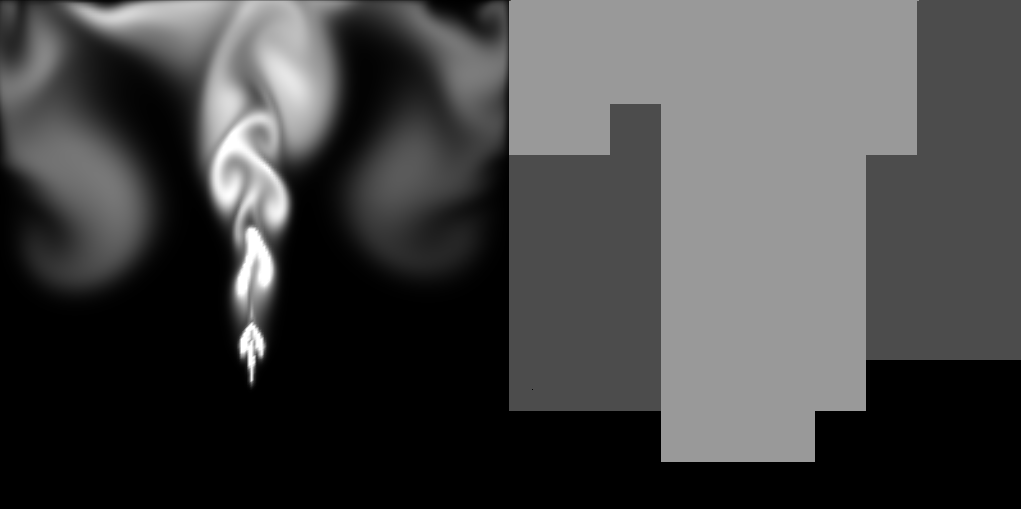
\includegraphics[scale=0.1]{img/logo.png} }

\subject{ Presentaci\'on Tesina 2017 } % \tiny{ }

\date{ \today} % \today will show
%current date.

\setbeamertemplate{navigation symbols}{}%remove navigation symbols 

%custom beaver footnote do what ever u want
\setbeamertemplate{footline} {%
\leavevmode
%
\hbox{%
\begin{beamercolorbox}[wd=.323\paperwidth,ht=2.25ex,dp=1ex,center]
    {author in head/foot}%
    \usebeamerfont{author in head/foot} Universidad Nacional de Rosario
\end{beamercolorbox}
%
\begin{beamercolorbox}[wd=.333\paperwidth,ht=2.25ex,dp=1ex,center]
    {title in head/foot}%
    \usebeamerfont{title in head/foot}\insertshorttitle
\end{beamercolorbox}
%
\begin{beamercolorbox}[wd=.3333\paperwidth,ht=2.25ex,dp=1ex,right]
    {date in head/foot}%
    \usebeamerfont{date in head/foot}\insertshortdate{}\hspace*{2em}
    \insertframenumber{} / \inserttotalframenumber\hspace*{1ex}
\end{beamercolorbox}
}%
\vskip0pt%
}

%\logo{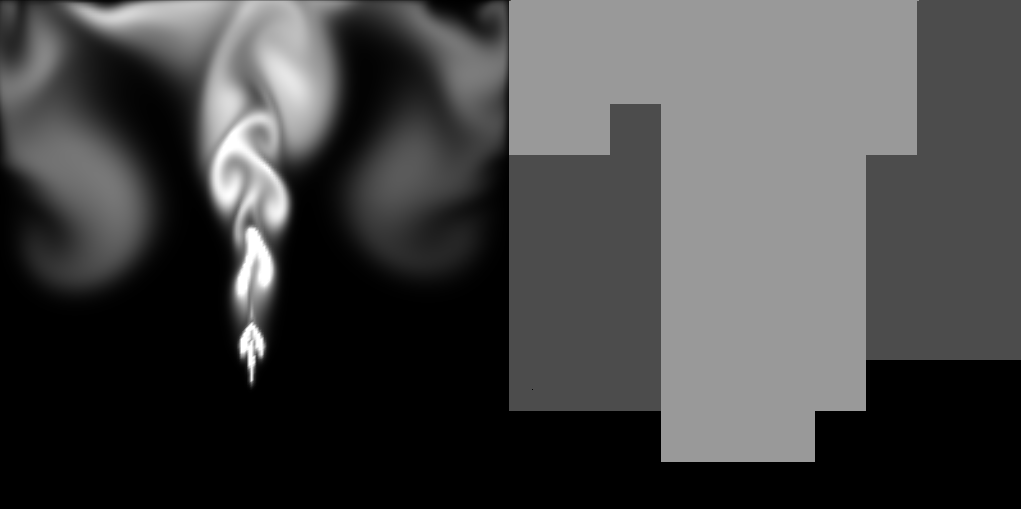
\includegraphics[scale=.04]{img/logo.png}}

\newcommand\codeHighlight[1]{\textcolor[rgb]{1,0,0}{\textbf{#1}}}

%~ \newenvironment{rcases} {\left.
%~ \begin{aligned}
    %~ } {%
%~ \end{aligned}
%~ \right\rbrace}

\lstset{escapeinside={<@}{@>}}

\begin{document}
%
{ \setbeamertemplate{logo}{}
\begin{frame}
    \titlepage
    \vspace*{-25px}
    \begin{center}
        \large{ Presentaci\'on de Tesina }
    \end{center}
\end{frame}
}

%%%%%%%%%%%%%%%%%%%%%%%%%%%%%%%%%%%%%%%%%%%%%%%%%%%%%%%%%%%%%%%%%%%%%%%%%%%%%%%%
\begin{frame}
    \frametitle{Introduccion}
    %more concrete simualtions, but a more abstract kind of problem
    \begin{itemize}
    \item
    Muchas aplicaciones de \textbf{cómputo intensivo} realizan
    \textbf{cálculos aproximados}
    \item 
    Algunas Razones: 
    \begin{itemize}
        \item
			para simular objetos o fenomenos del mundo real
		\item
			trabajan con sensores limitados en precision
		\item
			estan sometidas a un deadline de tiempo
		\item
			calculan resultados preliminares
    \end{itemize}
    \end{itemize}
\end{frame}
%%%%%%%%%%%%%%%%%%%%%%%%%%%%%%%%%%%%%%%%%%%%%%%%%%%%%%%%%%%%%%%%%%%%%%%%%%%%%%%%
\begin{frame}
\frametitle{Introduccion}
Algunos ejemplos de estas aplicaciones son: 
    \begin{itemize}
        \item
			Simulaciónes Físicas
		\item
			Sensores de entrada, algoritmos de procesamiento
		\item
			Decodificación de Video en tiempo real
		\item 
			Predicción de Terremotos
		\item 
			Aplicaciones de exploracion de geofisica
    \end{itemize}
    %~ Generalmente, estas aplicaciones necesitan una gran cantitdad de poder computacional.
   %~ \begin{figure} 
	 %~ 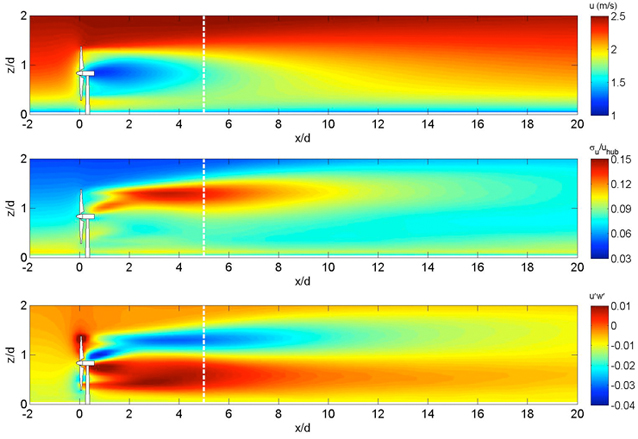
\includegraphics[scale=0.18]{img/wind_sim.jpg}
    %~ \end{figure}
\end{frame}
%%%%%%%%%%%%%%%%%%%%%%%%%%%%%%%%%%%%%%%%%%%%%%%%%%%%%%%%%%%%%%%%%%%%%%%%%%%%%%%%
\begin{frame}
\frametitle{Introduccion}
Normalmente, el desarrollo de estos 
algoritmos puede dividirse en \textbf{dos estapas}:
\begin{itemize}
\item Desarrollo de un kernel de computo ideal
	\begin{itemize} 
	\item ajuste del algoritmo
	\item debugueo
	\end{itemize}
\item Optimizacion a una version de produccion
	\begin{itemize}
	\item ajustando el nivel de precision para realizar calculos
	precisos solo donde es necesario
	\item escalar al tamano real del problema
	\item satisfacer un deadline
	\end{itemize}
\end{itemize}
\end{frame}
%%%%%%%%%%%%%%%%%%%%%%%%%%%%%%%%%%%%%%%%%%%%%%%%%%%%%%%%%%%%%%%%%%%%%%%%%%%%%%%%
\begin{frame}
\frametitle{Introduccion}
Optimizad un kernel ideal tiene complicaciones: 
\begin{itemize} 
\item es \textcolor{red}{complejo}
\item \textcolor{red}{lleva tiempo}
\item conduce a \textcolor{red}{codigos menos mantenibles}
\item hay que \textcolor{red}{hacerlo nuevamente} cuando hay cambios grandes en la estrategia
\end{itemize}
Esto se podria reducir con un \textbf{enfoque automatico de compilacion}
\end{frame}
%%%%%%%%%%%%%%%%%%%%%%%%%%%%%%%%%%%%%%%%%%%%%%%%%%%%%%%%%%%%%%%%%%%%%%%%%%%%%%%%
\begin{frame}
\frametitle{Introduccion}
	Existen enfoques automaticos de optimizacion para computo intensivo:
	\begin{itemize}
	\item manteniendo la semantica original
	\begin{itemize}
		\item paralelizacion
		\item localidad de datos
		\item vectorizacion
	\end{itemize}
	\textcolor{blue}{bien abordados por los compiladores}
	\item modificando la semantica original
	\begin{itemize}
		\item relajacion de dependencias
		\item modificiacion o eliminacion de calculos
		\item usando conocimiento especifico de dominio 
	\end{itemize} 
	\textcolor{red}{escasamente abordados por los compiladores}
	\end{itemize}
\end{frame}
%%%%%%%%%%%%%%%%%%%%%%%%%%%%%%%%%%%%%%%%%%%%%%%%%%%%%%%%%%%%%%%%%%%%%%%%%%%%%%%%
\begin{frame}
\frametitle{Introduccion}

Para aplicaciones que calculan resultados aproximados, un enfoque automatico 
de optimizacion que modifique la semantica original es adecuado siempre
que asegure una \textbf{precision aceptable}.

\end{frame} 
%%%%%%%%%%%%%%%%%%%%%%%%%%%%%%%%%%%%%%%%%%%%%%%%%%%%%%%%%%%%%%%%%%%%%%%%%%%%%%%%
\begin{frame}
\frametitle{Introduccion}
\textbf{Nuestro Objetivo}: Busacar formas de optimizar codigos que computan
aproximaciones 
\begin{itemize} 
\item de forma \textbf{automatica}
\item \textbf{modificando la semantica} original
\item asegurando una \textbf{precision aceptable} 
\end{itemize}
\end{frame}
%%%%%%%%%%%%%%%%%%%%%%%%%%%%%%%%%%%%%%%%%%%%%%%%%%%%%%%%%%%%%%%%%%%%%%%%%%%%%%%%
\begin{frame}
\frametitle{Introduccion}
Para realizarlo utilizaremos
\begin{itemize} 
\item El \textbf{Modelo Poliedrico} para realizar transformaciones agresivas de codigo
\item \textbf{Conocimiento de Dominio Especifico} suministrado por el usuario
	\begin{itemize} 
	\item que guie la transformacion de codigo	
	\item mantenga una precision aceptable
\end{itemize}
\item Un enfoque \textbf{adaptivo}
	\begin{itemize} 
		\item realiza calculos complejos solamente donde es necesario
		\item ahorra computaciones que no impactan en el resultado
		\item transforma el codigo de forma dinamica
	\end{itemize}
\end{itemize}
\end{frame}
%%%%%%%%%%%%%%%%%%%%%%%%%%%%%%%%%%%%%%%%%%%%%%%%%%%%%%%%%%%%%%%%%%%%%%%%%%%%%%%%
\begin{frame} 
\frametitle{Contenido} 
\begin{itemize}
\item \textbf{Transformacion de Codigo: Modelo Poliedrico}
\item Herramienta estatica: Spot
\item Refinamiento Adaptivo de Codigo
\item Experimentos con Simulacion de Fluidos
\item Conclusiones y Trabajo Futuro
\end{itemize}
\end{frame} 
%%%%%%%%%%%%%%%%%%%%%%%%%%%%%%%%%%%%%%%%%%%%%%%%%%%%%%%%%%%%%%%%%%%%%%%%%%%%%%%%
\begin{frame} 
\frametitle{Modelo Poliedrico}
	\begin{itemize} 
	\item Es un modelo matematico-computacional para la optimizacion y 
			paralelizacion automatica de programas
	\item muy poderoso para la representacion y transformacion estructural de programas
	\item Representa bucles matematicamente con \textbf{relaciones afines}
		\begin{itemize}
		\item dominios de iteracion
		\item relaciones de orden
		\item relaciones de acceso
		\end{itemize}
	\end{itemize}
		\begin{figure}
			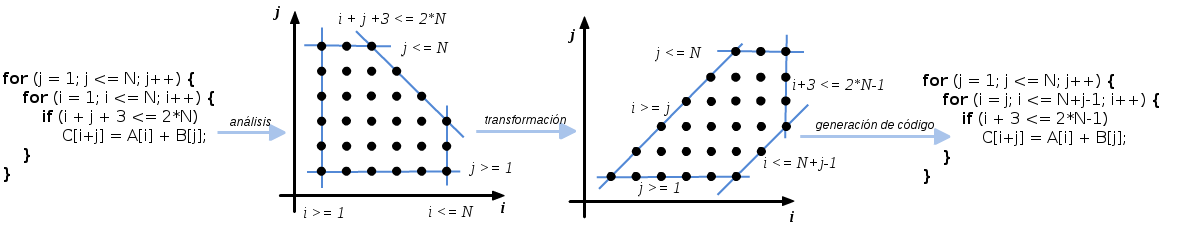
\includegraphics[scale=0.30]{img/poly_pipeline2.png}
		\end{figure}
\end{frame}
%%%%%%%%%%%%%%%%%%%%%%%%%%%%%%%%%%%%%%%%%%%%%%%%%%%%%%%%%%%%%%%%%%%%%%%%%%%%%%%%
\begin{frame}[fragile]
\frametitle{Dominios de Iteracion}
\begin{itemize}
\item \textbf{instancia de statement}: una ejecucion individual de un stamement $S$ 
\item $S(i',j')$ es la instancia de $S$ para los valores $i=i'$ y $j=j'$ 
\item el \textbf{dominio de iteracion} queda definido por el conjunto de valores
del vector $\left(\begin{smallmatrix}i\\j\\\end{smallmatrix}\right)$
\item el dominio de iteracion se puede representar con un \textbf{poliedro} 
\end{itemize}
\begin{columns}
\column[t]{0.55\textwidth}
\begin{figure}
\begin{lstlisting}[basicstyle=\scriptsize,language=C]
    for (i = 0; i < 2 * N - 1; i++) 
S1:     z[i] = 0;
        
    for (i = 0; i < N; i++) 
        for (j = 0; j < N; j++)
S2:         <@\textcolor{violet}{z[i+j] = x[i] + y[j];} @>
\end{lstlisting}
\caption{multiplicacion de matrices}
\end{figure}
\column[t]{0.45\textwidth}
\begin{figure}
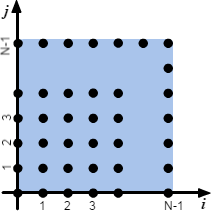
\includegraphics[scale=0.4]{img/poly_mul_solo.png}
\caption{instancias de $S2$}
\end{figure}
\end{columns}
\end{frame}
%%%%%%%%%%%%%%%%%%%%%%%%%%%%%%%%%%%%%%%%%%%%%%%%%%%%%%%%%%%%%%%%%%%%%%%%%%%%%%%%
\begin{frame}
\frametitle{Representacion poliedrica: Dominios de Iteracion}
\begin{columns}
\column[t]{0.45\textwidth}
inecuaciones del dominio de iteracion de $S2$: 
\begin{itemize}
\item $ i \geq 0 $
\item $ i  < N $
\item $ j \geq 0 $
\item $ j < N $
\end{itemize}
\column[t]{0.45\textwidth}
ecuacion matricial: 
$$
\begin{bmatrix*}[r] 1 &  0 & 0 &  0 \\ 
                               -1 &  0 & 1 & -1 \\ 
                                0 &  1 & 0 &  0 \\
                                0 & -1 & 1 & -1 \end{bmatrix*} 
            \left( \begin{array}{c} i \\ j \\ N\\ 1\\ \end{array} \right)
            \geq \vec{0}
$$
\end{columns}
\begin{itemize}
\item representacion \textcolor{blue}{poderosa y compacta} 
\item \textcolor{red}{restricciones}:
\begin{itemize}
\item no hay esquema general para soportar flujo de control dinamico
\item cotas de bucles y condicionales \textcolor{red}{deben ser funciones afines}
de iteradores exteriores y parametros
\end{itemize}
\end{itemize} 
\end{frame}
%%%%%%%%%%%%%%%%%%%%%%%%%%%%%%%%%%%%%%%%%%%%%%%%%%%%%%%%%%%%%%%%%%%%%%%%%%%%%%%%
\begin{frame}[fragile]
\frametitle{Representacion poliedrica: Relaciones de Ordenamiento y Posicion }
\begin{itemize}
\item especifican \textbf{orden y lugar} de cada instancia
\item \textbf{orden}: posicion temporal de ejecucion con respecto
otras instancias
\item \textbf{lugar}: en que procesador deben ejecutarse
\item a cada instancia se le asigna una \textbf{fecha logica}
\begin{columns}
\column[t]{0.40\textwidth}
\begin{equation}
\nonumber
\theta_{S_1}(N, i) = \left(\begin{matrix} 0 \\ i\\\end{matrix} \right)
\end{equation}
\begin{equation}
\nonumber
\theta_{S_2}(N, i, j) =  \left(\begin{matrix} 1 \\ i \\ j \\\end{matrix} \right)
\end{equation}
\column[t]{0.55\textwidth}
\begin{figure}
\begin{lstlisting}[basicstyle=\scriptsize,language=C]
    for (i = 0; i < 2 * N - 1; i++) 
S1:     z[i] = 0;
        
    for (i = 0; i < N; i++) 
        for (j = 0; j < N; j++)
S2:         z[i+j] = x[i] + y[j];
\end{lstlisting}
\end{figure}
\vfill \null
\end{columns}
\item los statements se ejecutan en \textcolor{blue}{orden lexicografico} 
\item \textcolor{red}{las funciones de ordenamiento deben ser afines}
\end{itemize}
\end{frame}
%%%%%%%%%%%%%%%%%%%%%%%%%%%%%%%%%%%%%%%%%%%%%%%%%%%%%%%%%%%%%%%%%%%%%%%%%%%%%%%%
\begin{frame}
\frametitle{Representacion poliedrica: Relaciones de Ordenamiento y Posicion}
relaciones afines: 
$$
{\scriptstyle
 \theta_{S_1}(N) = 
        \left\{ 
            \left(\begin{matrix}i\\\end{matrix} \right) \to 
            \left(\begin{matrix}t_1 \\ t_2\\\end{matrix} \right) 
            \in \mathbb{Z} \times \mathbb{Z}^2  \middle|
            \begin{bmatrix*}[r] -1 &  0 & 0 &  0 & 0 \\ 
                                0  & -1 & 1 &  0 & 0  \end{bmatrix*} 
            \left( \begin{array}{c} t_1 \\ t_2 \\ i \\ N \\ 1\\ \end{array} \right)
            = \vec{0}
        \right\},
}
$$ 
$$
{\scriptstyle
 \theta_{S_2}(N) = 
        \left\{ 
            \left(\begin{matrix}i \\ j \\\end{matrix} \right) \to 
            \left(\begin{matrix}t_1 \\ t_2 \\ t_3 \\\end{matrix} \right) 
            \in \mathbb{Z}^2 \times \mathbb{Z}^3  \middle|
            \begin{bmatrix*}[r] -1 &  0 &  0 & 0 &  0 & 0 & 1 \\ 
                                0  & -1 &  0 & 1 &  0 & 0 & 0 \\
                                0  &  0 & -1 & 0 &  1 & 0 & 0 \end{bmatrix*} 
            \left( \begin{array}{c} t_1 \\ t_2 \\ t_3 \\ i \\ j \\ N \\ 1\\ \end{array} \right)
            = \vec{0}
        \right\}
}
$$

\end{frame}
%%%%%%%%%%%%%%%%%%%%%%%%%%%%%%%%%%%%%%%%%%%%%%%%%%%%%%%%%%%%%%%%%%%%%%%%%%%%%%%%
\begin{frame}
\frametitle{Representacion Poliedrica: Funciones de Acceso}

\end{frame}
%%%%%%%%%%%%%%%%%%%%%%%%%%%%%%%%%%%%%%%%%%%%%%%%%%%%%%%%%%%%%%%%%%%%%%%%%%%%%%%%



\begin{frame}
\frametitle{}

\end{frame}
%%%%%%%%%%%%%%%%%%%%%%%%%%%%%%%%%%%%%%%%%%%%%%%%%%%%%%%%%%%%%%%%%%%%%%%%%%%%%%%%


% End of slides
\end{document}
 


